\section{Dataset Overview}
\label{sec:Dataset Overview}
The CINIC-10 dataset combines images from CIFAR-10 and downsampled ImageNet organized into the three standard splits of \texttt{train}, \texttt{valid}, 
and \texttt{test}. Each split contains an equal number of $32 \times 32$ color images from the same ten object categories \textit{airplane}, 
\textit{automobile}, \textit{bird}, \textit{cat}, \textit{deer}, \textit{dog}, \textit{frog}, \textit{horse}, \textit{ship} and \textit{truck}.
Each class in each split consists of 2000 CIFAR-10 images and 7000 ImageNet images, resulting in a total of 9000 images per class per split.

\subsection{Preprocessing}
To enable our domain classification task we first annotated each image with a \texttt{source} label. This label was inferred directly from the 
image filename. CIFAR-10 images have filenames starting with \texttt{cifar-10}, while ImageNet-derived images begin with \texttt{n} or a numeric 
identifier. This naming convention was inferred from the README file of the CINIC-10 GitHub repository~\cite{cinic10_github}. These labels were 
added to a metadata table stored as a CSV file.
Each row in the resulting metadata file contains:
\begin{itemize}
  \item \texttt{split}: one of \texttt{train}, \texttt{valid} or \texttt{test}
  \item \texttt{category}: the object class label (e.g., \textit{cat}, \textit{truck})
  \item \texttt{filename} and \texttt{full\_path}: the image filename and relative path
  \item \texttt{source}: either \texttt{CIFAR-10} or \texttt{ImageNet}
\end{itemize}
For training, all images were normalized to the $[0, 1]$ range by dividing pixel values by 255.
We also implemented a custom data generator class to load batches of images on demand during training, reducing memory usage and supporting 
efficient training on large datasets. This generator reads image paths and labels from the CSV files, loads them in batches, applies preprocessing, 
and yields image-label pairs to the model.

This setup allows the training of both deep learning and classical machine learning models on the exact same data structure, ensuring fair 
comparisons and reproducible results.

\subsection{Examples and Visualizations}
\label{subsec:Examples and Visualizations}

To illustrate the characteristics and distribution of the CINIC-10 dataset, we include a set of visualizations and image examples.

Figure~\ref{fig:class-distribution} shows the distribution of images per class and source in the 
CINIC-10 dataset. Each class in each split contains exactly 9000 images, but the internal composition of those classes is imbalanced with 7000
images coming from ImageNet and 2000 from CIFAR-10. This imbalance could influence model learning and needs to be accounted for during 
evaluation.

\begin{figure}[H]
    \centering
    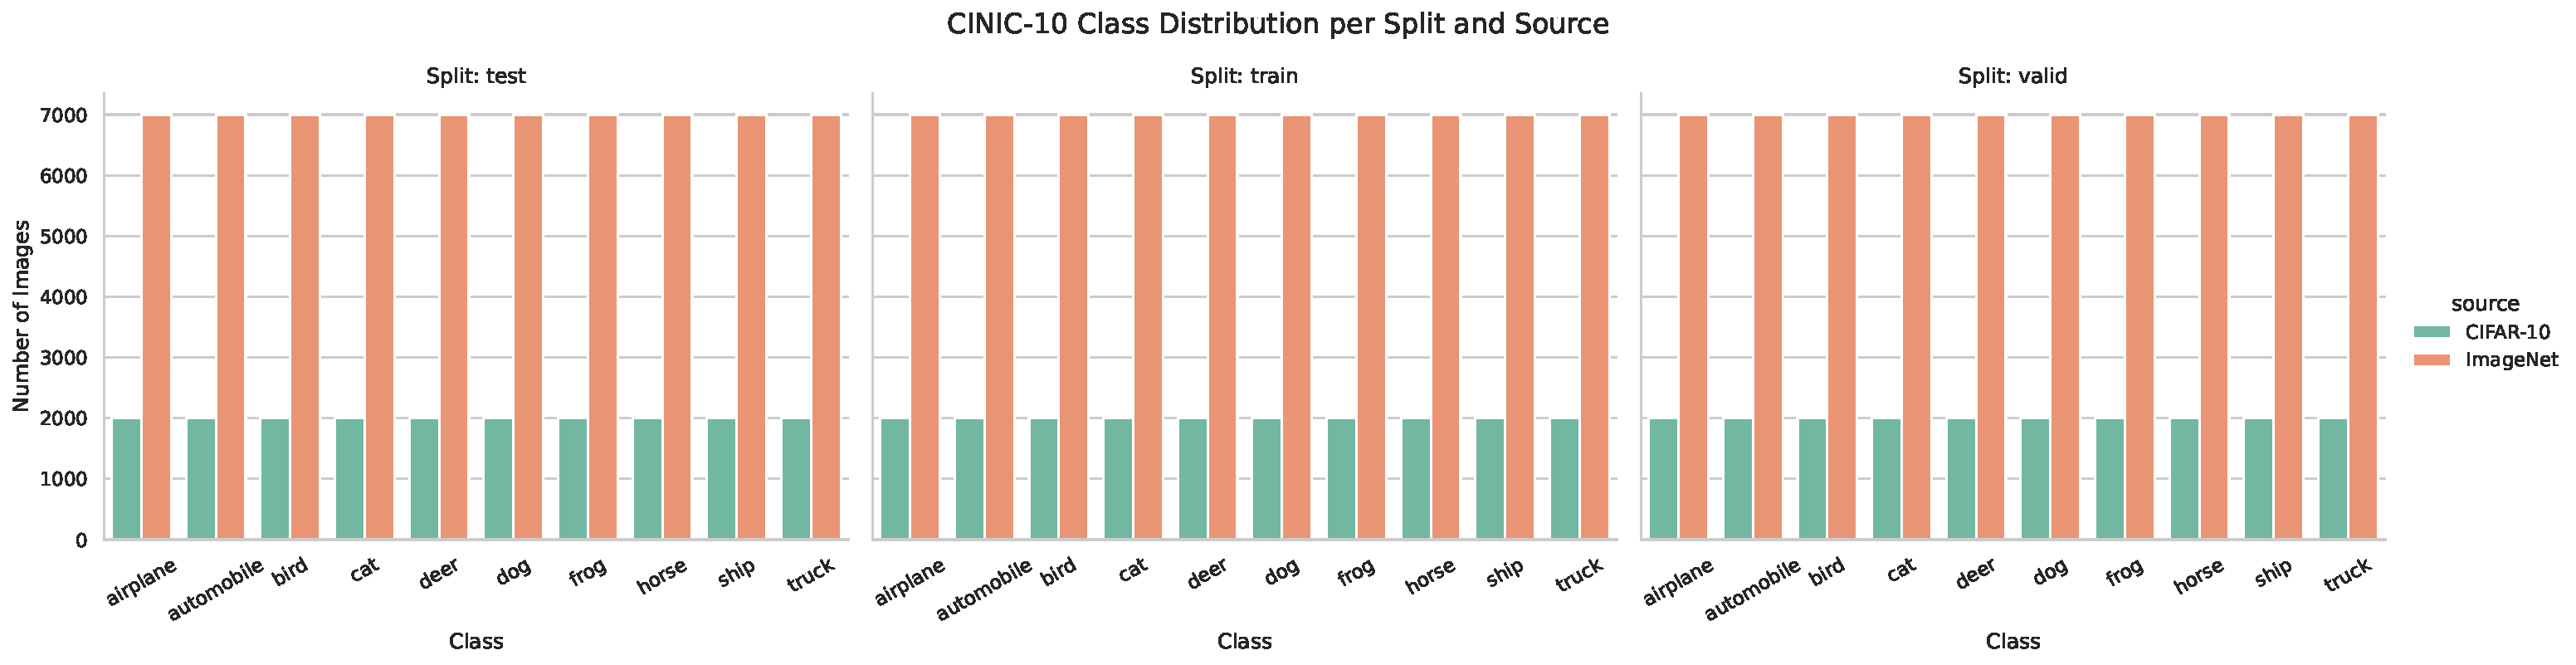
\includegraphics[width=0.95\textwidth]{Plots/DatasetOverview/cinic10_class_distribution.pdf}
    \caption{Distribution of classes and sources in the CINIC-10 dataset. Each class contains 9,000 images per split, but within each class, CIFAR-10 contributes 2,000 images and ImageNet 7,000.}
    \label{fig:class-distribution}
\end{figure}

In Figure~\ref{fig:rgb-stats}, we compare the mean and variance of RGB channel values per class, 
separated by source. While the differences appear small at first glance, they are systematic and consistent across categories. This suggests the 
presence of subtle domain-specific color or lighting distributions, which models might exploit when distinguishing between sources.

\begin{figure}[H]
    \centering
    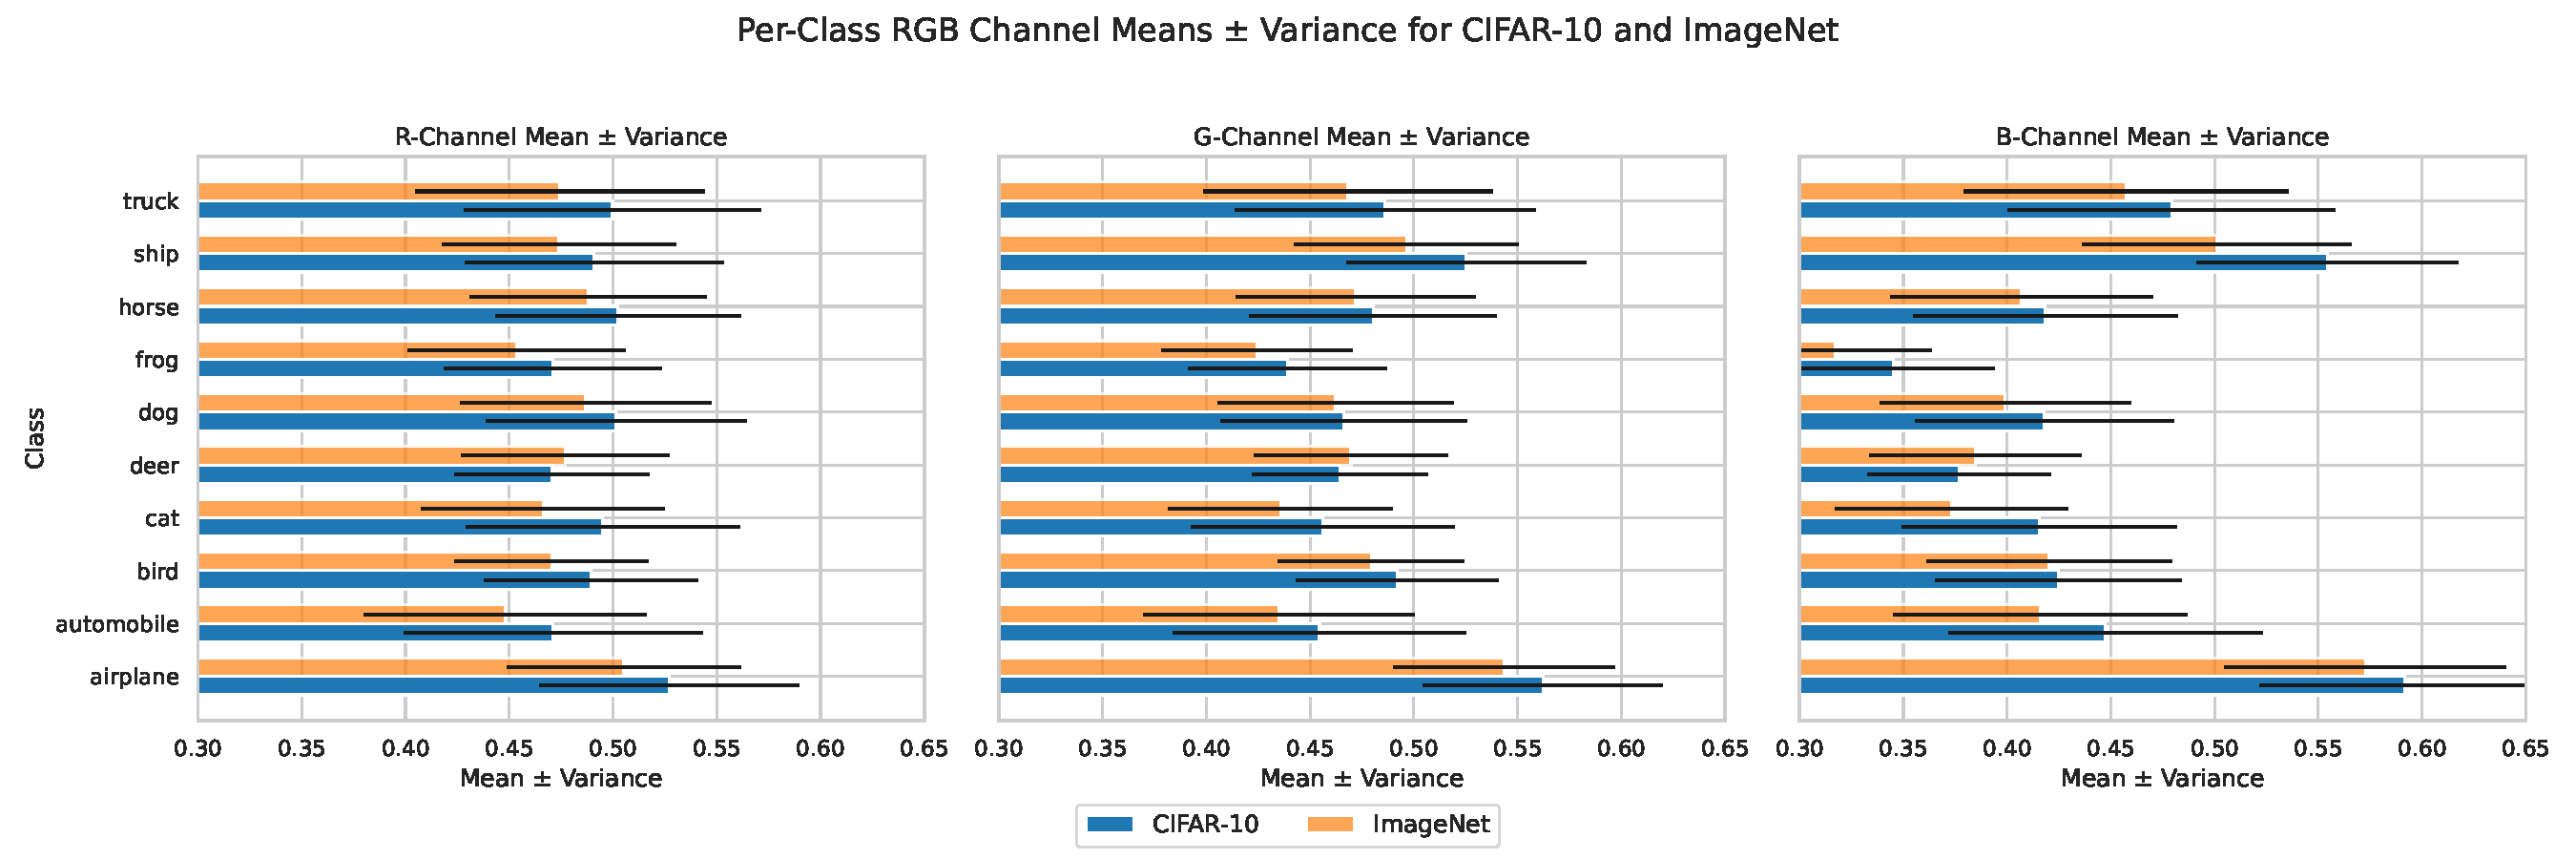
\includegraphics[width=0.95\textwidth]{Plots/DatasetOverview/rgb_means_variance_per_class.pdf}
    \caption{Mean and variance of RGB channels for each class, separated by source. Small but consistent differences between CIFAR-10 and ImageNet images are observable.}
    \label{fig:rgb-stats}
\end{figure}

To complement these quantitative statistics, we show concrete examples from the dataset. Figure~\ref{fig:automobile-comparison}
presents a comparison of the \textit{automobile} class from CIFAR-10 and ImageNet. CIFAR-10 images are visually uniform, typically centered and 
consistently lit. Imagenet appears to be mostly the same even though I can remember a remark at University that Cifar looks more "stockfootagy". 

To complement the quantitative results, we include visual examples from the dataset. Figure~\ref{fig:automobile-comparison} compares samples from the \textit{automobile} class in CIFAR-10 and ImageNet. While both sets feature centered and well-lit vehicles, CIFAR-10 images often appear more uniform and curated. This impression, sometimes likened to "stock footage," may partly result from prolonged exposure to similar, looking images during analysis.

Figure~\ref{fig:dog-comparison} shows examples from the \textit{dog} class. Again, CIFAR-10 
and ImageNet images appear to look simliar. Interestingly, the final image in the ImageNet row appears to be a 
fox, which highlights the presence of mislabeled or ambiguous samples in the dataset, as previously discussed by Northcutt et al.~\cite
{northcutt2021confident}.

\begin{figure}[H]
    \centering
    \begin{subfigure}[b]{\textwidth}
        \centering
        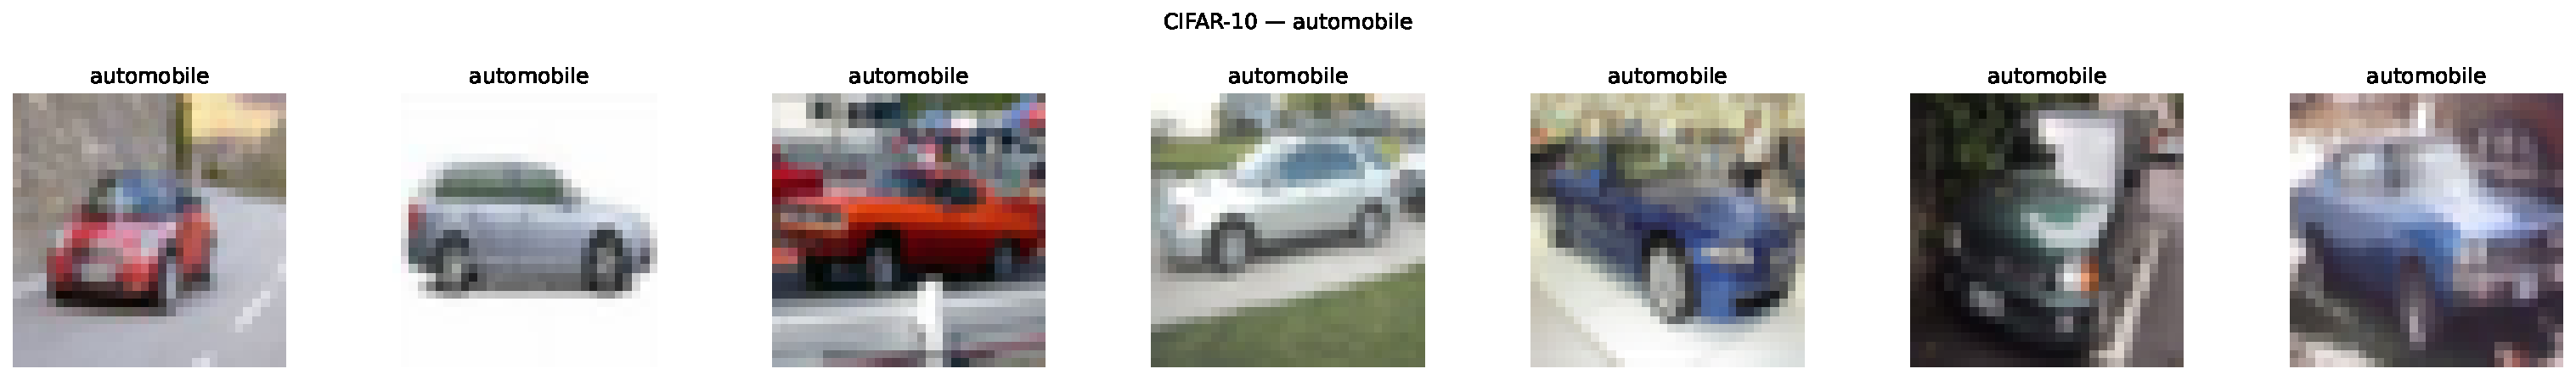
\includegraphics[width=\textwidth]{Plots/DatasetOverview/cifar_automobile_7_grid.pdf}
        \caption{CIFAR-10: \textit{automobile} class}
        \label{fig:cifar-automobile}
    \end{subfigure}

    \begin{subfigure}[b]{\textwidth}
        \centering
        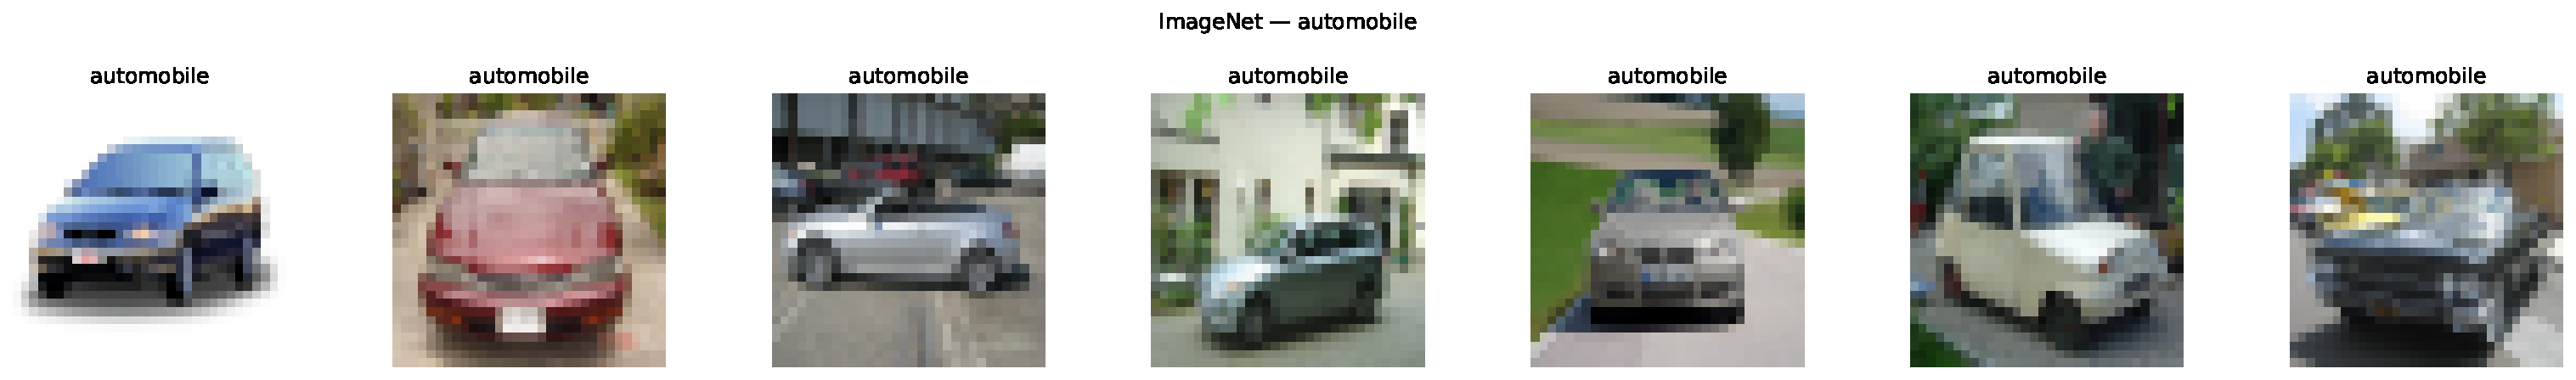
\includegraphics[width=\textwidth]{Plots/DatasetOverview/imageNet_automobile_7_grid.pdf}
        \caption{ImageNet: \textit{automobile} class}
        \label{fig:imagenet-automobile}
    \end{subfigure}
    
    \caption{Example images from the \textit{automobile} class in both CIFAR-10 and ImageNet.}
    \label{fig:automobile-comparison}
\end{figure}


\begin{figure}[H]
    \centering
    \begin{subfigure}[b]{\textwidth}
        \centering
        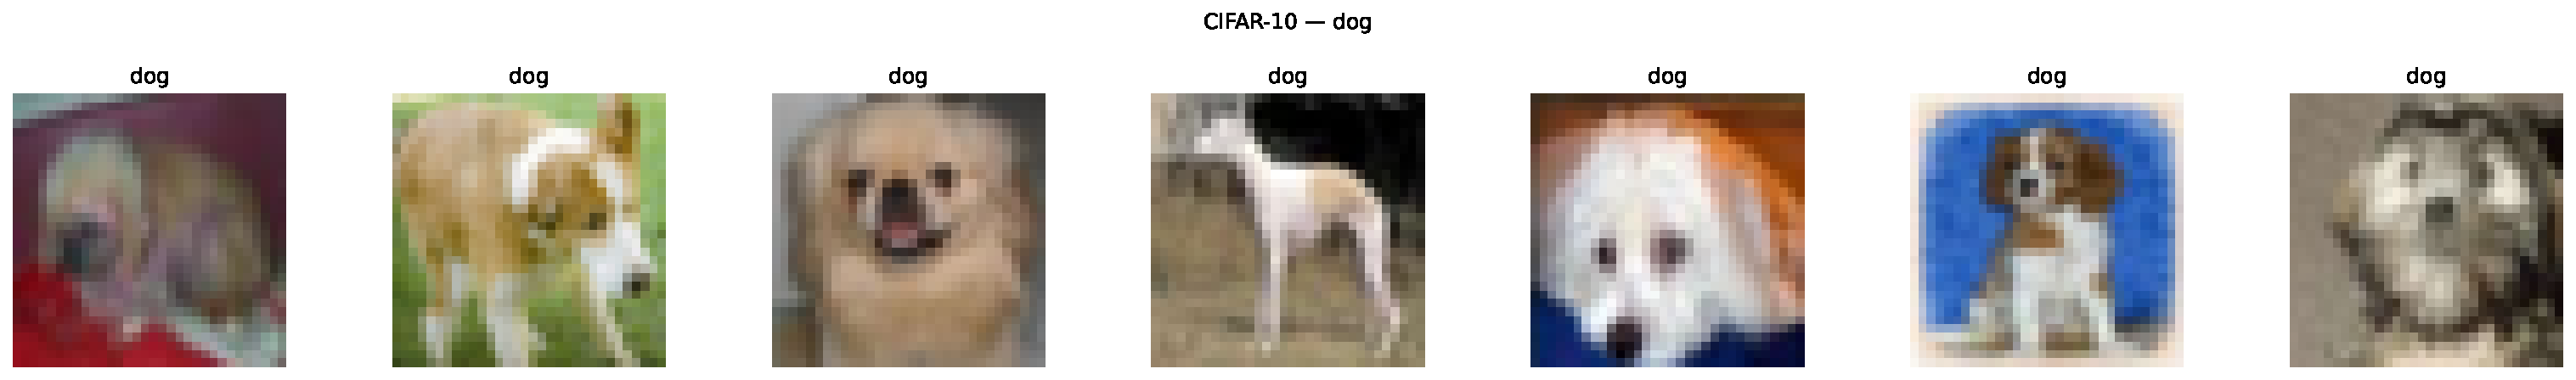
\includegraphics[width=\textwidth]{Plots/DatasetOverview/cifar_dog_7_grid.pdf}
        \caption{CIFAR-10: \textit{dog} class}
        \label{fig:cifar-dog}
    \end{subfigure}

    \begin{subfigure}[b]{\textwidth}
        \centering
        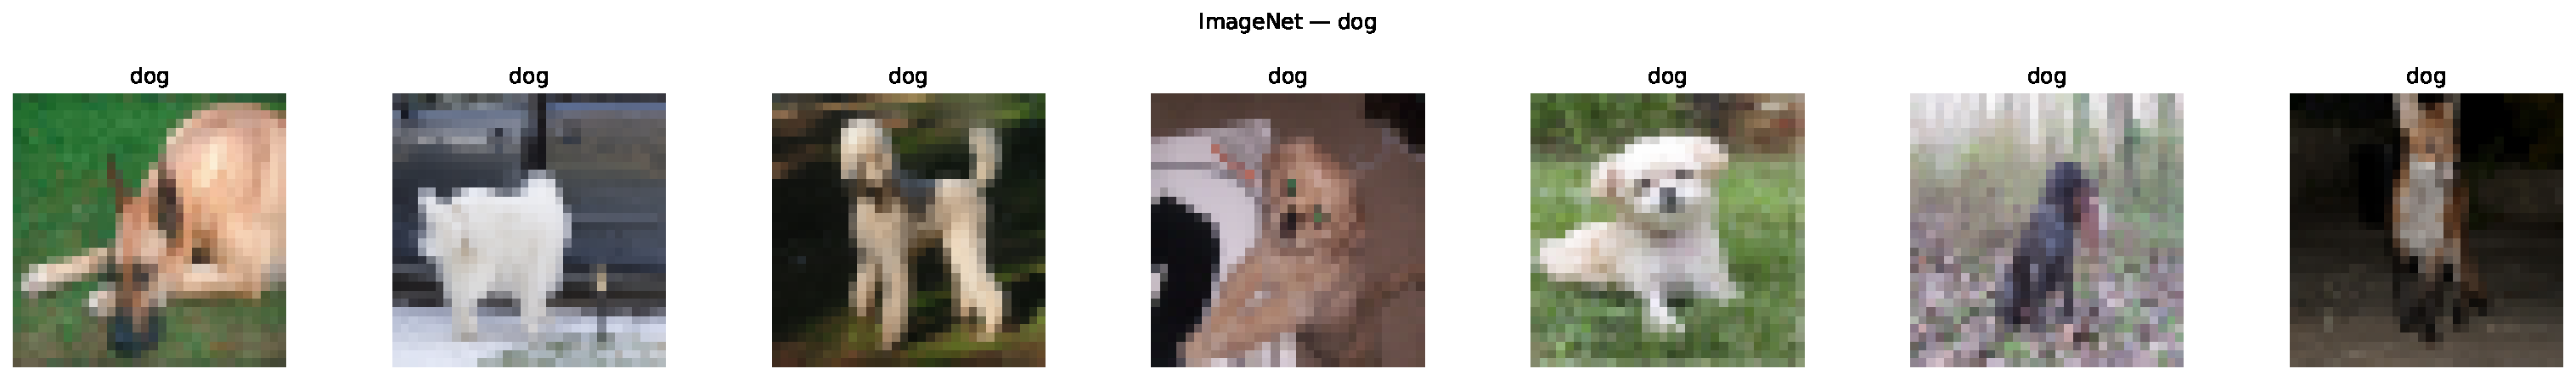
\includegraphics[width=\textwidth]{Plots/DatasetOverview/imageNet_dog_7_grid.pdf}
        \caption{ImageNet: \textit{dog} class}
        \label{fig:imagenet-dog}
    \end{subfigure}
    
    \caption{Example images from the \textit{dog} class in CIFAR-10 and ImageNet. Notably, the last ImageNet example appears to depict a fox, illustrating the presence of mislabeled data in the dataset as discussed in \cite{northcutt2021confident}.}
    \label{fig:dog-comparison}
\end{figure}

These visual and statistical comparisons highlight not only the domain differences between CIFAR-10 and ImageNet but also the types of cues a model 
might use to differentiate between them.
